% GNUPLOT: LaTeX picture with Postscript
\begingroup
  \makeatletter
  \providecommand\color[2][]{%
    \GenericError{(gnuplot) \space\space\space\@spaces}{%
      Package color not loaded in conjunction with
      terminal option `colourtext'%
    }{See the gnuplot documentation for explanation.%
    }{Either use 'blacktext' in gnuplot or load the package
      color.sty in LaTeX.}%
    \renewcommand\color[2][]{}%
  }%
  \providecommand\includegraphics[2][]{%
    \GenericError{(gnuplot) \space\space\space\@spaces}{%
      Package graphicx or graphics not loaded%
    }{See the gnuplot documentation for explanation.%
    }{The gnuplot epslatex terminal needs graphicx.sty or graphics.sty.}%
    \renewcommand\includegraphics[2][]{}%
  }%
  \providecommand\rotatebox[2]{#2}%
  \@ifundefined{ifGPcolor}{%
    \newif\ifGPcolor
    \GPcolortrue
  }{}%
  \@ifundefined{ifGPblacktext}{%
    \newif\ifGPblacktext
    \GPblacktexttrue
  }{}%
  % define a \g@addto@macro without @ in the name:
  \let\gplgaddtomacro\g@addto@macro
  % define empty templates for all commands taking text:
  \gdef\gplbacktext{}%
  \gdef\gplfronttext{}%
  \makeatother
  \ifGPblacktext
    % no textcolor at all
    \def\colorrgb#1{}%
    \def\colorgray#1{}%
  \else
    % gray or color?
    \ifGPcolor
      \def\colorrgb#1{\color[rgb]{#1}}%
      \def\colorgray#1{\color[gray]{#1}}%
      \expandafter\def\csname LTw\endcsname{\color{white}}%
      \expandafter\def\csname LTb\endcsname{\color{black}}%
      \expandafter\def\csname LTa\endcsname{\color{black}}%
      \expandafter\def\csname LT0\endcsname{\color[rgb]{1,0,0}}%
      \expandafter\def\csname LT1\endcsname{\color[rgb]{0,1,0}}%
      \expandafter\def\csname LT2\endcsname{\color[rgb]{0,0,1}}%
      \expandafter\def\csname LT3\endcsname{\color[rgb]{1,0,1}}%
      \expandafter\def\csname LT4\endcsname{\color[rgb]{0,1,1}}%
      \expandafter\def\csname LT5\endcsname{\color[rgb]{1,1,0}}%
      \expandafter\def\csname LT6\endcsname{\color[rgb]{0,0,0}}%
      \expandafter\def\csname LT7\endcsname{\color[rgb]{1,0.3,0}}%
      \expandafter\def\csname LT8\endcsname{\color[rgb]{0.5,0.5,0.5}}%
    \else
      % gray
      \def\colorrgb#1{\color{black}}%
      \def\colorgray#1{\color[gray]{#1}}%
      \expandafter\def\csname LTw\endcsname{\color{white}}%
      \expandafter\def\csname LTb\endcsname{\color{black}}%
      \expandafter\def\csname LTa\endcsname{\color{black}}%
      \expandafter\def\csname LT0\endcsname{\color{black}}%
      \expandafter\def\csname LT1\endcsname{\color{black}}%
      \expandafter\def\csname LT2\endcsname{\color{black}}%
      \expandafter\def\csname LT3\endcsname{\color{black}}%
      \expandafter\def\csname LT4\endcsname{\color{black}}%
      \expandafter\def\csname LT5\endcsname{\color{black}}%
      \expandafter\def\csname LT6\endcsname{\color{black}}%
      \expandafter\def\csname LT7\endcsname{\color{black}}%
      \expandafter\def\csname LT8\endcsname{\color{black}}%
    \fi
  \fi
  \setlength{\unitlength}{0.0500bp}%
  \begin{picture}(9070.00,4534.00)%
    \gplgaddtomacro\gplbacktext{%
      \csname LTb\endcsname%
      \put(1078,704){\makebox(0,0)[r]{\strut{}-20}}%
      \put(1078,1150){\makebox(0,0)[r]{\strut{}-17.5}}%
      \put(1078,1595){\makebox(0,0)[r]{\strut{}-15}}%
      \put(1078,2041){\makebox(0,0)[r]{\strut{}-12.5}}%
      \put(1078,2487){\makebox(0,0)[r]{\strut{}-10}}%
      \put(1078,2932){\makebox(0,0)[r]{\strut{}-7.5}}%
      \put(1078,3378){\makebox(0,0)[r]{\strut{}-5}}%
      \put(1078,3823){\makebox(0,0)[r]{\strut{}-2.5}}%
      \put(1078,4269){\makebox(0,0)[r]{\strut{} 0}}%
      \put(1210,484){\makebox(0,0){\strut{}-20}}%
      \put(2143,484){\makebox(0,0){\strut{}-17.5}}%
      \put(3076,484){\makebox(0,0){\strut{}-15}}%
      \put(4009,484){\makebox(0,0){\strut{}-12.5}}%
      \put(4941,484){\makebox(0,0){\strut{}-10}}%
      \put(5874,484){\makebox(0,0){\strut{}-7.5}}%
      \put(6807,484){\makebox(0,0){\strut{}-5}}%
      \put(7740,484){\makebox(0,0){\strut{}-2.5}}%
      \put(8673,484){\makebox(0,0){\strut{} 0}}%
      \csname LTb\endcsname%
      \put(176,2486){\rotatebox{-270}{\makebox(0,0){\strut{}$\,$$\widehat{v}_{z,IMP,0,analytical}$$[\frac{ft}{sec}]$}}}%
      \put(4941,154){\makebox(0,0){\strut{}$\,$$v_{z,IMP,0}$ $[\frac{ft}{sec}]$}}%
      \put(5389,2201){\makebox(0,0)[l]{\strut{}$FAR_{total}$}}%
      \put(7292,2201){\makebox(0,0)[l]{\strut{}$=9.20\%$}}%
      \put(5389,1916){\makebox(0,0)[l]{\strut{}$FAR_{DST\, \& \,SST}$}}%
      \put(7292,1916){\makebox(0,0)[l]{\strut{}$=2.96\%$}}%
      \put(5389,1631){\makebox(0,0)[l]{\strut{}$FAR_{DST}$}}%
      \put(7292,1631){\makebox(0,0)[l]{\strut{}$=0.00\%$}}%
      \put(5389,1346){\makebox(0,0)[l]{\strut{}$FAR_{SST}$}}%
      \put(7292,1346){\makebox(0,0)[l]{\strut{}$=6.24\%$}}%
      \put(2068,3289){\makebox(0,0)[l]{\strut{}$MAR_{total}$=1.3\%}}%
      \put(2068,2183){\makebox(0,0)[l]{\strut{}$DR_{total}=96\%$}}%
    }%
    \gplgaddtomacro\gplfronttext{%
    }%
    \gplbacktext
    \put(0,0){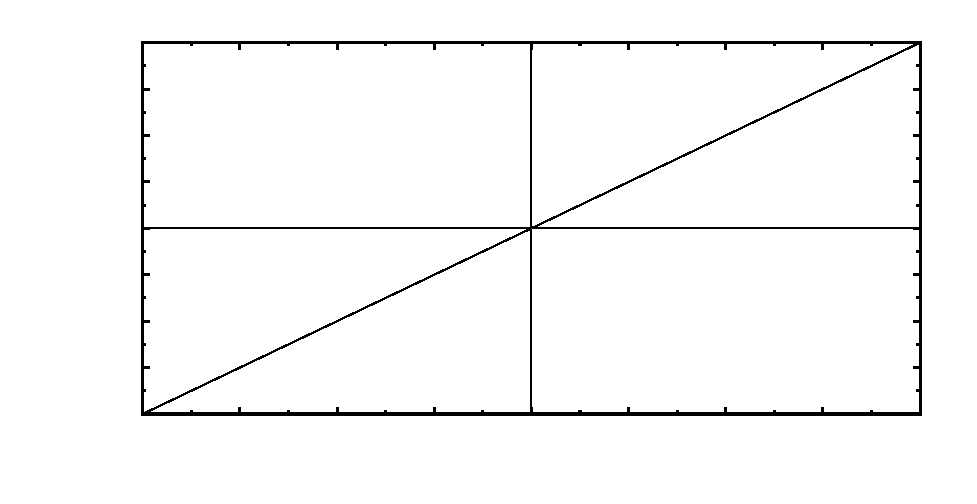
\includegraphics{global_performance}}%
    \gplfronttext
  \end{picture}%
\endgroup
